%%%%%%%%%%%%%%%%%%%%%%%%%%%%%%%%%%%%%%%%%%%%%%%
%%%This is a science homework template. Modify the preamble to suit your needs. 
%The junk text is   there for you to immediately see how the headers/footers look at first 
%typesetting.


\documentclass[answers,11pt]{exam}

%AMS-TeX packages
\usepackage{amssymb,amsmath,amsthm}
%geometry (sets margin) and other useful packages
\usepackage{alltt}
\usepackage{booktabs}
\usepackage{enumerate}
\usepackage{fullpage}
\usepackage{graphicx,ctable,booktabs}
\usepackage{hyperref}
\newcommand{\h}{\widehat}

%
%Redefining sections as problems
%
\makeatletter
\newenvironment{problem}{\@startsection
       {section}
       {1}
       {-.2em}
       {-3.5ex plus -1ex minus -.2ex}
       {2.3ex plus .2ex}
       {\pagebreak[3]%forces pagebreak when space is small; use \eject for better results
       \large\bf\noindent{Problem }
       }
       }
       {%\vspace{1ex}\begin{center} \rule{0.3\linewidth}{.3pt}\end{center}}
       \begin{center}\large\bf \ldots\ldots\ldots\end{center}}
\makeatother



\DeclareMathOperator*{\sd}{sd}


%
%Fancy-header package to modify header/page numbering 
%
%\usepackage{fancyhdr}
%\pagestyle{fancy}
%\addtolength{\headwidth}{\marginparsep} %these change header-rule width
%\addtolength{\headwidth}{\marginparwidth}
%\lhead{Problem \thesection}
%\chead{} 
%\rhead{\thepage} 
%\lfoot{\small\scshape course name}
%\cfoot{} 
%\rfoot{\footnotesize HW \#1}
%\renewcommand{\headrulewidth}{.3pt}
%\renewcommand{\footrulewidth}{.3pt}
%\setlength\voffset{-0.25in}
%\setlength\textheight{648pt}

%%%%%%%%%%%%%%%%%%%%%%%%%%%%%%%%%%%%%%%%%%%%%%%

%
%Contents of problem set
%    
\begin{document}

\begin{center}
  \large
  \textbf{Homework \#5 -- Due Tuesday, Aug.~7} \\
  STAT-UB.0001 -- Statistics for Business Control \\
\end{center}


\thispagestyle{empty}

\begin{problem}{}

For each of the following values of $\alpha$, and $n$, find $t_{\alpha/2,n-1}$. 
Round the answer to two digits after the decimal point.

\begin{enumerate}[(a)]

\item $\alpha = 0.10$, $n = 25$.
    \begin{solution}
        \[
            t_{.050,24} = 1.711 \approx 1.71.
        \]
    \end{solution}


\item $\alpha = 0.02$, $n = 10$.
    \begin{solution}
        \[
            t_{.010,9} = 2.821 \approx 2.82.
        \]
    \end{solution}


\end{enumerate}

\end{problem}

\begin{problem}{}

Consider the time it takes for a call center to answer its calls. A random
sample of $7$ calls revealed a sample mean time of $191$ seconds and a sample
standard deviation of $11.4$ seconds.

\begin{enumerate}[(a)]

\item What is the sample?
    \begin{solution}
        The times to answer the $n = 7$ sampled calls.
    \end{solution}
\item What is the population?
    \begin{solution}
The times to answer all calls at the call center.
    \end{solution}
\item Explain what the population mean represents in this problem.
    \begin{solution}
The expected time it takes the call center to answer a call.  (Equivalently,
the average of all of the times taken to answer all calls at the call center.)
    \end{solution}
\item Construct a 95\% confidence interval for the population mean.
    \begin{solution}
For a 95\% confidence interval and $7$ observations, we have $\alpha = .05$
and
\[
  t_{\alpha/2,n-1} = t_{.025,6} = 2.447.
\]
The 95\% confidence interval for the population mean is
\begin{align*}
  \bar x \pm t_{\alpha/2,n-1} \frac{s}{\sqrt{n}}
    &= 191 \pm 2.447 \frac{11.4}{\sqrt{7}} \\
    &= 191 \pm 10.5 \\
    &= (180.5, 201.5).
\end{align*}

    \end{solution}

\item Construct a 99\% confidence interval for the population mean.
    \begin{solution}
For a 99\% confidence interval and $7$ observations, we have $\alpha = .01$
and
\[
  t_{\alpha/2,n-1} = t_{.005,6} = 3.707.
\]
The 99\% confidence interval for the population mean is
\begin{align*}
  \bar x \pm t_{\alpha/2,n-1} \frac{s}{\sqrt{n}}
    &= 191 \pm 3.707 \frac{11.4}{\sqrt{7}} \\
    &= 191 \pm 16 \\
    &= (175, 207).
\end{align*}
    \end{solution}

\item State any assumptions you needed to do this problem. Do you think that
the assumptions are reasonable? Why or why not?
    \begin{solution}
Since the sample size is small ($n < 30$), we need to assume that the
population is normal.  That is, we need to assume that the histogram of the
times to answer all calls looks like a bell curve.  Personally, I do not think
that this is reasonable; I expect that the time to answer a call has a high
skew to the right.  (You will still get full credit if you think that the
assumption is reasonable, as your reasoning makes sense.)
    \end{solution}

\end{enumerate}

\end{problem}

\begin{problem}{}

Consider (again) the time it takes for a call center to answer its calls. Assume the 
time to answer a call is normally distributed.  
The call center claims that the mean time to answer a call is $3$ minutes.  In a
random sample of $7$ calls, the average time for the call center to answer was
$191$ seconds, with a sample standard deviation of $11.4$ seconds.

\begin{enumerate}[(a)]


\item Provide the null and alternative hypotheses for testing the call
center's claim.
    \begin{solution}
Let $\mu$ be the population mean.
\begin{align*}
  H_0 &: \mu = 180 \\
  H_a &: \mu \neq 180.
\end{align*}


    \end{solution}
\item Compute the test statistic.
    \begin{solution}
The sample size is $n = 7$.  The sample mean and standard deviation are
$\bar x = 191$ and $s = 11.4$.  The hypothesized null mean is $\mu_0 = 180$.

\begin{align*}
  t &= \frac{\bar x - \mu_0}{s/\sqrt{n}} \\
    &= \frac{191 - 180}{11.4/\sqrt{7}} \\
    &= 2.55 
\end{align*}
    \end{solution}

\item Compute the $p$-value.
    \begin{solution}
We will approximate the $p$-value using a $z$ table:

\begin{align*}
  p &\approx P(|Z| > 2.55) \\
    &= 0.009322
\end{align*}
Note that the value $z = 2.55$ is not in the $Z$-table, so we use the value
for $z = 2.6$ instead.  It would be acceptable to use $z = 2.5$ instead, in
which case you would get $p \approx 0.01242$.

(A more accurate solution would use a $t$ distribution with $n - 1 = 6$
degrees of freedom; this gives a $p$-value of $p = 0.04349$.)

    \end{solution}

\item Test the call center's claim, at the 1\% level of significance.
    \begin{solution}
Since $p \geq 0.01$, we do not reject $H_0$.  The data is consistent with the
claim.

    \end{solution}

\end{enumerate}

\end{problem}



\begin{problem}{}
    You would like to estimate the proportion of Stern students who participates in course faculty evaluations (CFEs). 
    If you want to construct a 95\% confidence interval for this proportion, how many students should you survey 
    to guarantee that the width of your confidence interval will be less than 0.05?
    \textit{Hint: use the fact that $\h p (1-\h p) \leq \frac{1}{4}$, for any $\h p$ taking values between $[0,1]$.}

    \begin{solution}
        Suppose you sampled $n$ students, and the sample proportion of participating in CFE is $\h p$. 
        The 95\% CI for the population proportion is 
        \[
            \left(\h p -2\sqrt{\frac{\h p(1-\h p)}{n}}, 
            \h p +2\sqrt{\frac{\h p(1-\h p)}{n}}\right).
        \]
        The width of this CI is therefore $4 \sqrt{\frac{\h p(1-\h p)}{n}}$, which is upper bounded by
        \[
            4 \sqrt{\frac{\h p(1-\h p)}{n}} \leq 4 \sqrt{\frac{1}{4n}} = \frac{2}{\sqrt{n}} .
        \]
        To ensure that the width is less than $0.05$, 
        it is sufficient to have 
        \[
            \frac{2}{\sqrt{n}} \leq 0.05 \Rightarrow n \geq 1600. 
        \]
        Therefore you need to survey at least $1600$ students to ensure that 
        the width of your 95\% confidence interval will be less than 0.05. 
    \end{solution}

\end{problem}

\begin{problem}{}

Consider the \texttt{HeightWeight.csv} file containing data on 200 records of human heights and weights of 18 years
old children. Here, we focus on the the Weight (in lb) column. Use Minitab to complete the following questions.

\begin{enumerate}[(a)]

\item \label{part:weight-minitab} Use \textit{Stat $\Rightarrow$ Basic Statistics $\Rightarrow$ 1-Sample
t}, and choose \texttt{Weight} to create a
95\% confidence interval for the population mean.

\begin{solution}
\begin{center}
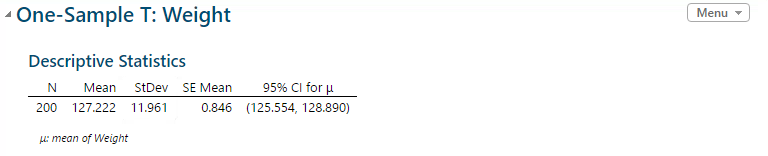
\includegraphics[width=0.8\textwidth]{5a.png}
\end{center}
\end{solution}
\item Use the Minitab output (\texttt{N}, \texttt{Mean}, \texttt{StDev}) to check the calculation of the confidence
interval in (\ref{part:weight-minitab}).  Also verify the calculation
of \texttt{SE Mean}, the (estimated) standard deviation for the sample mean.
\begin{solution}
We have 
\begin{align*}
& n=200, \bar x = 127.222, s=11.961\\
& z_{0.025}=1.96 \\
& 1.96 \frac{11.961}{\sqrt{200}} = 1.658\\
& \bar x \pm 1.658 = (125.56, 128.88)
\end{align*}
The CI is close to Minitab output (up to rounding errors).
\end{solution}

\item \label{part:weight-confint-99} Get a 99\% confidence interval for the population mean, proceeding as in
(\ref{part:weight-minitab}) but adding \textit{Options $\Rightarrow$
Confidence Level:} 99.0.

\begin{solution}
\begin{center}
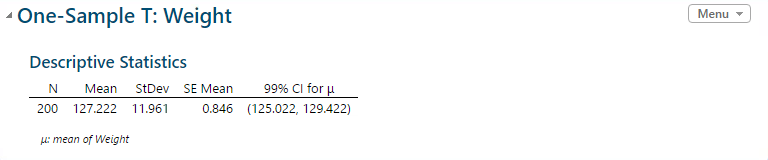
\includegraphics[width=0.8\textwidth]{5c.png}
\end{center}
\end{solution}
\item  According to Wikipedia, the average weight for adults is 136.7 lb. 
    Use Minitab to get the $p$-value corresponding to the null hypothesis that the average weight for the 18 years old children is the same as
    the average weight of the adults. Interpret the $p$-value.  Proceed as in (\ref{part:weight-minitab}) but select \textit{Perform hypothesis test}.
    \begin{solution}
\begin{center}
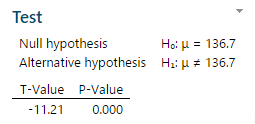
\includegraphics[width=0.3\textwidth]{5d.png}
\end{center}
The p-value is less than $0.05$, so we reject the null hypothesis that 18 years old children have the same average weight as adults.

\end{solution}
\end{enumerate}

\end{problem}



\end{document}


